\newpage
\section{Sqaending delay function: Delay of 2}

\begin{figure}[hb]
 %   \includegraphics[trim=2 10 14 4, clip]{figures/v_AllFig-DelayOf_2-Sqaending.png}    
    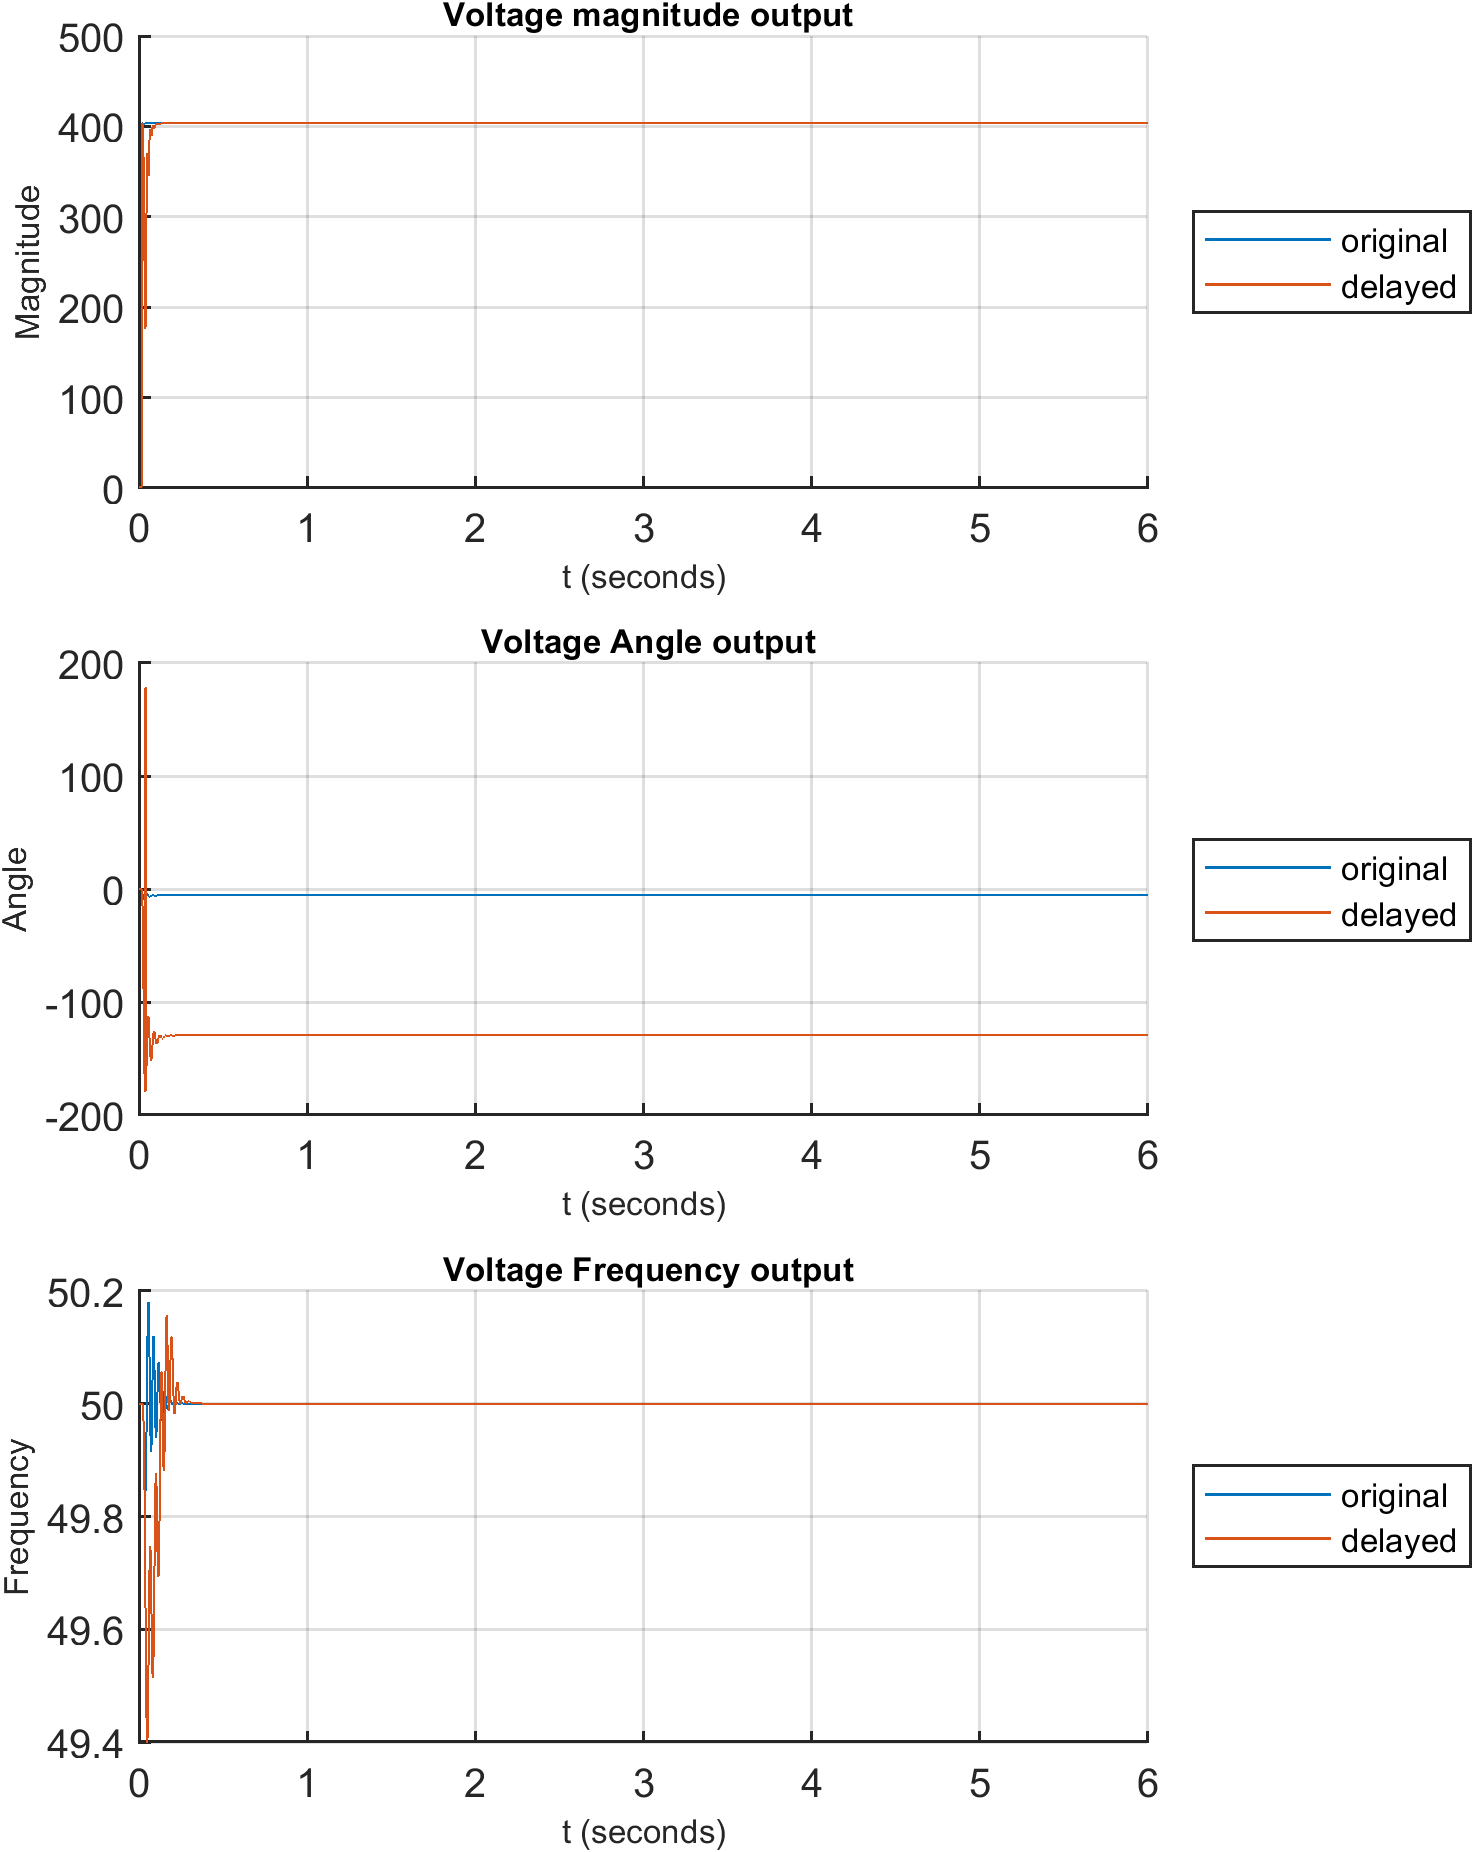
\includegraphics[width=0.95\textwidth]{\locateResults/AllFig.png}    
    \caption{Sqaending delay combined output}
    \label{fig:PMUsim-Sqa2-allfig}
\end{figure}


     \begin{figure}
 
    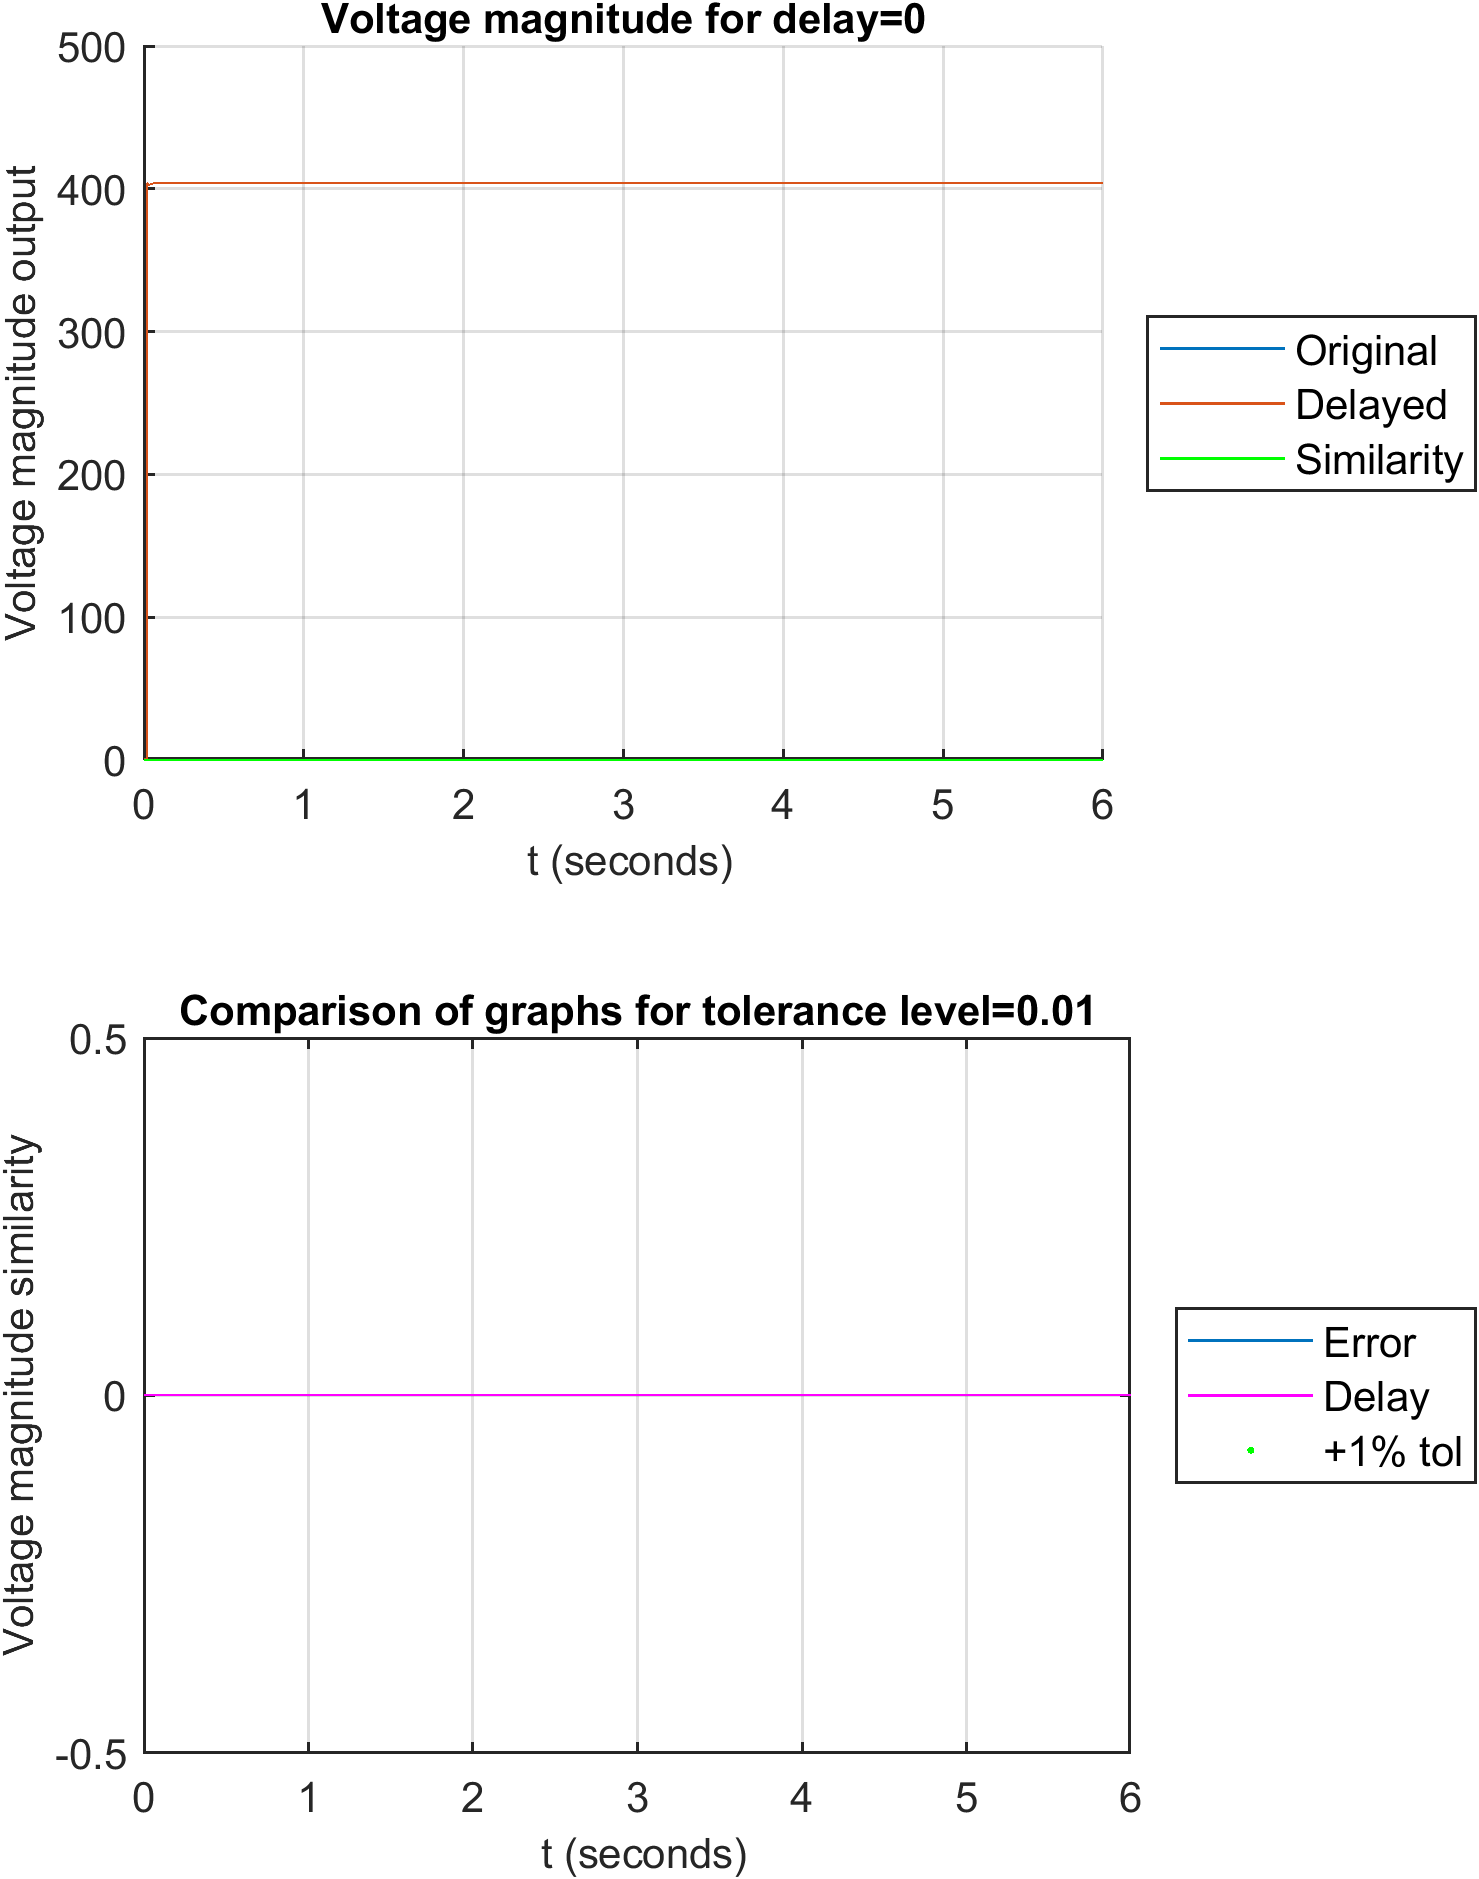
\includegraphics[width=\textwidth]{\locateResults/Magnitude.png}    
         %\caption{magnitude Output}
         \label{fig:PMUsim-Sqa2Mag}
        \caption{Magnitude component output}
 
\end{figure}

     \begin{figure}
 
   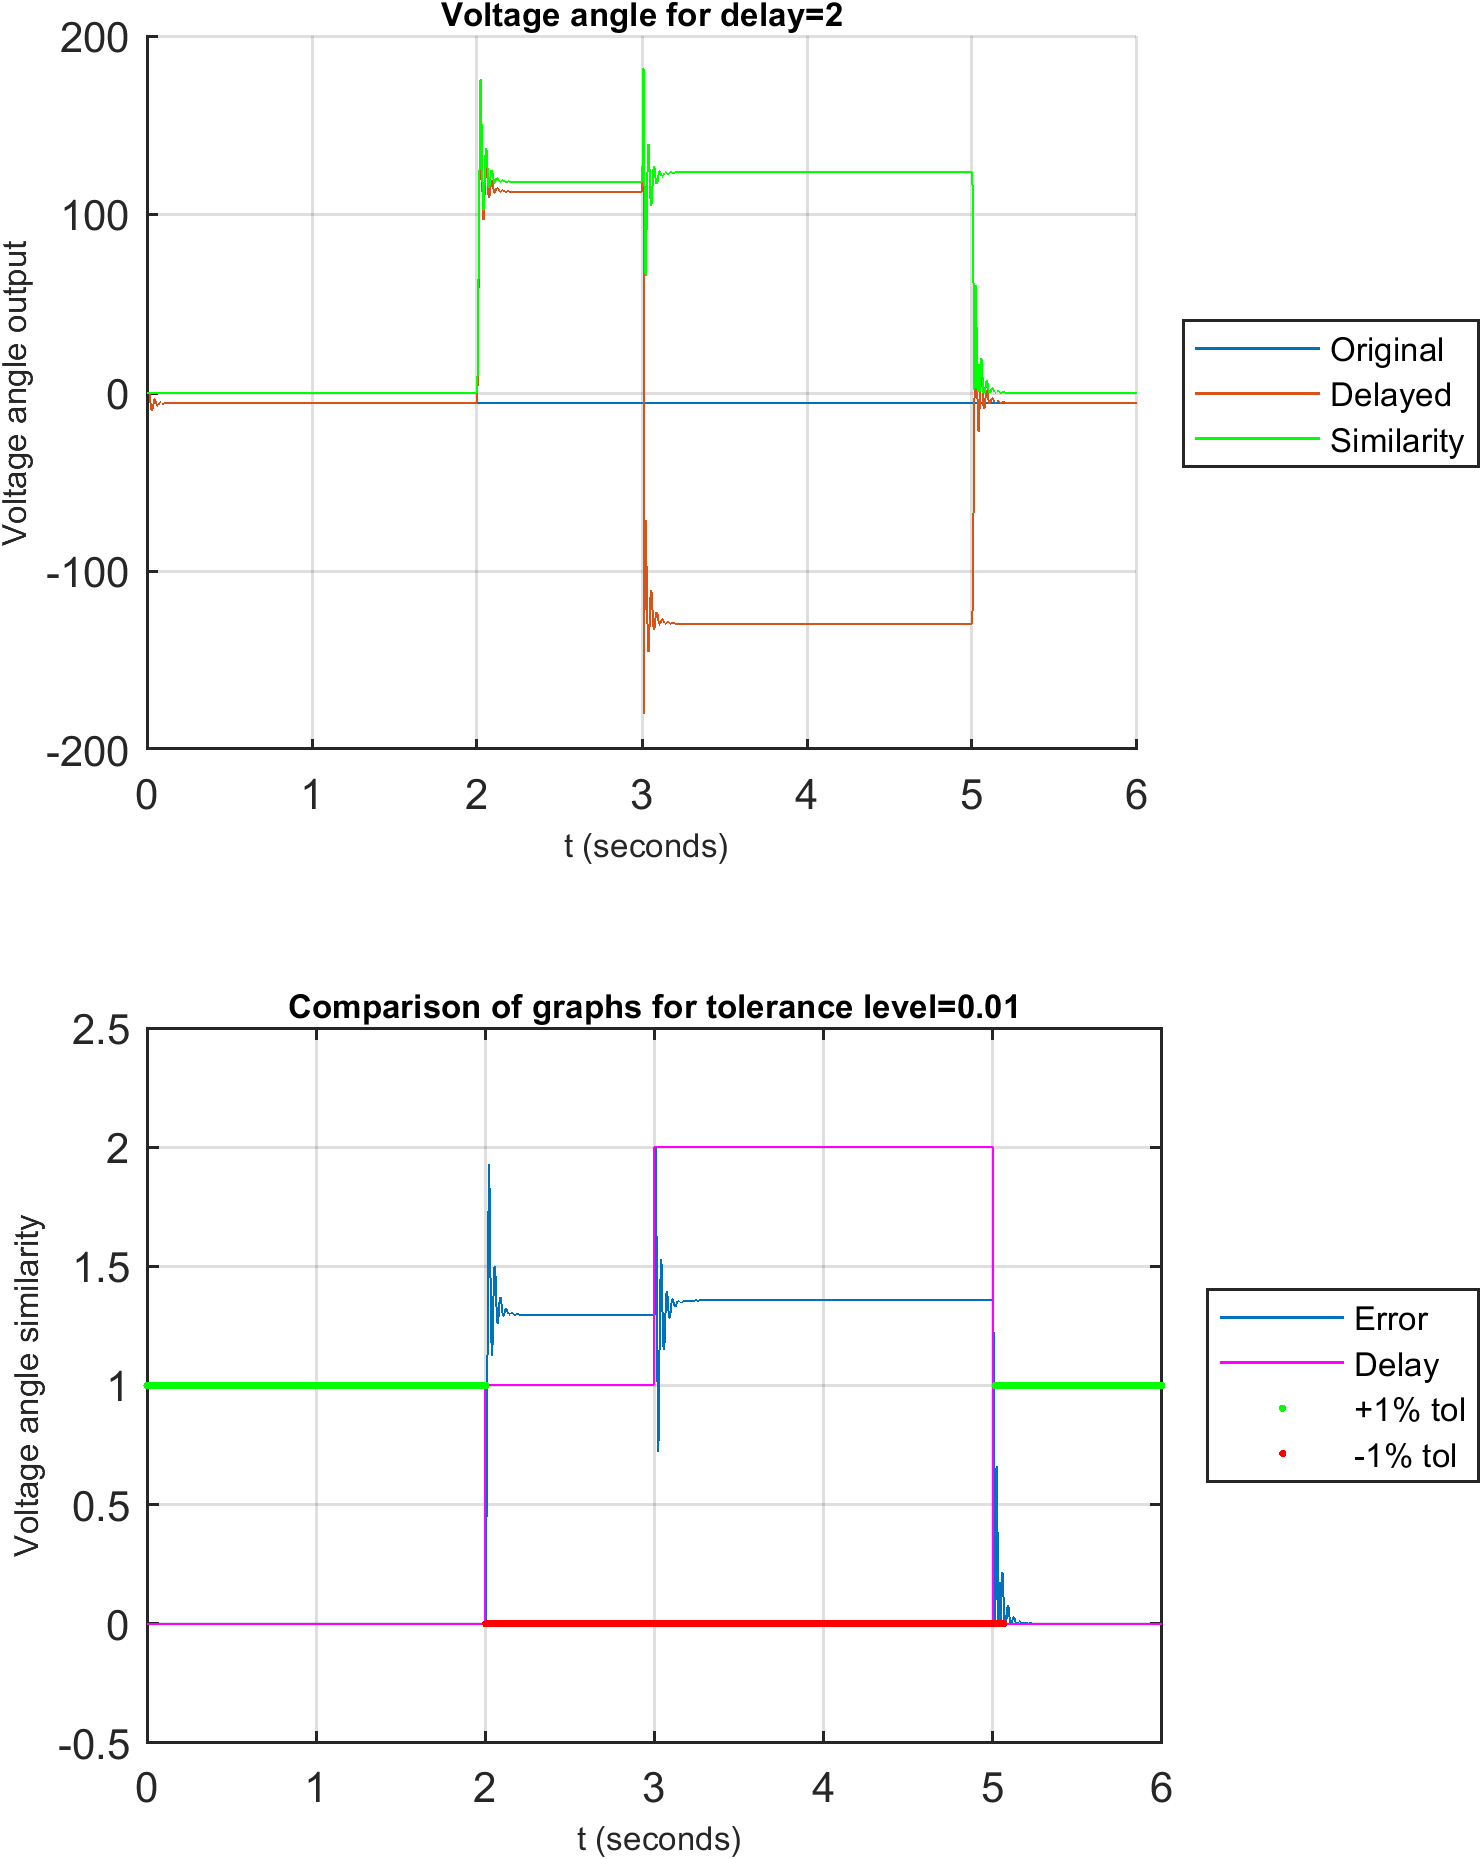
\includegraphics[width=\textwidth]{\locateResults/Angle.png}    
          %\caption{Angle Output}
         \label{fig:PMUsim-Sqa2Ang}
        \caption{Angle component output}
 
\end{figure}

     \begin{figure}
 
   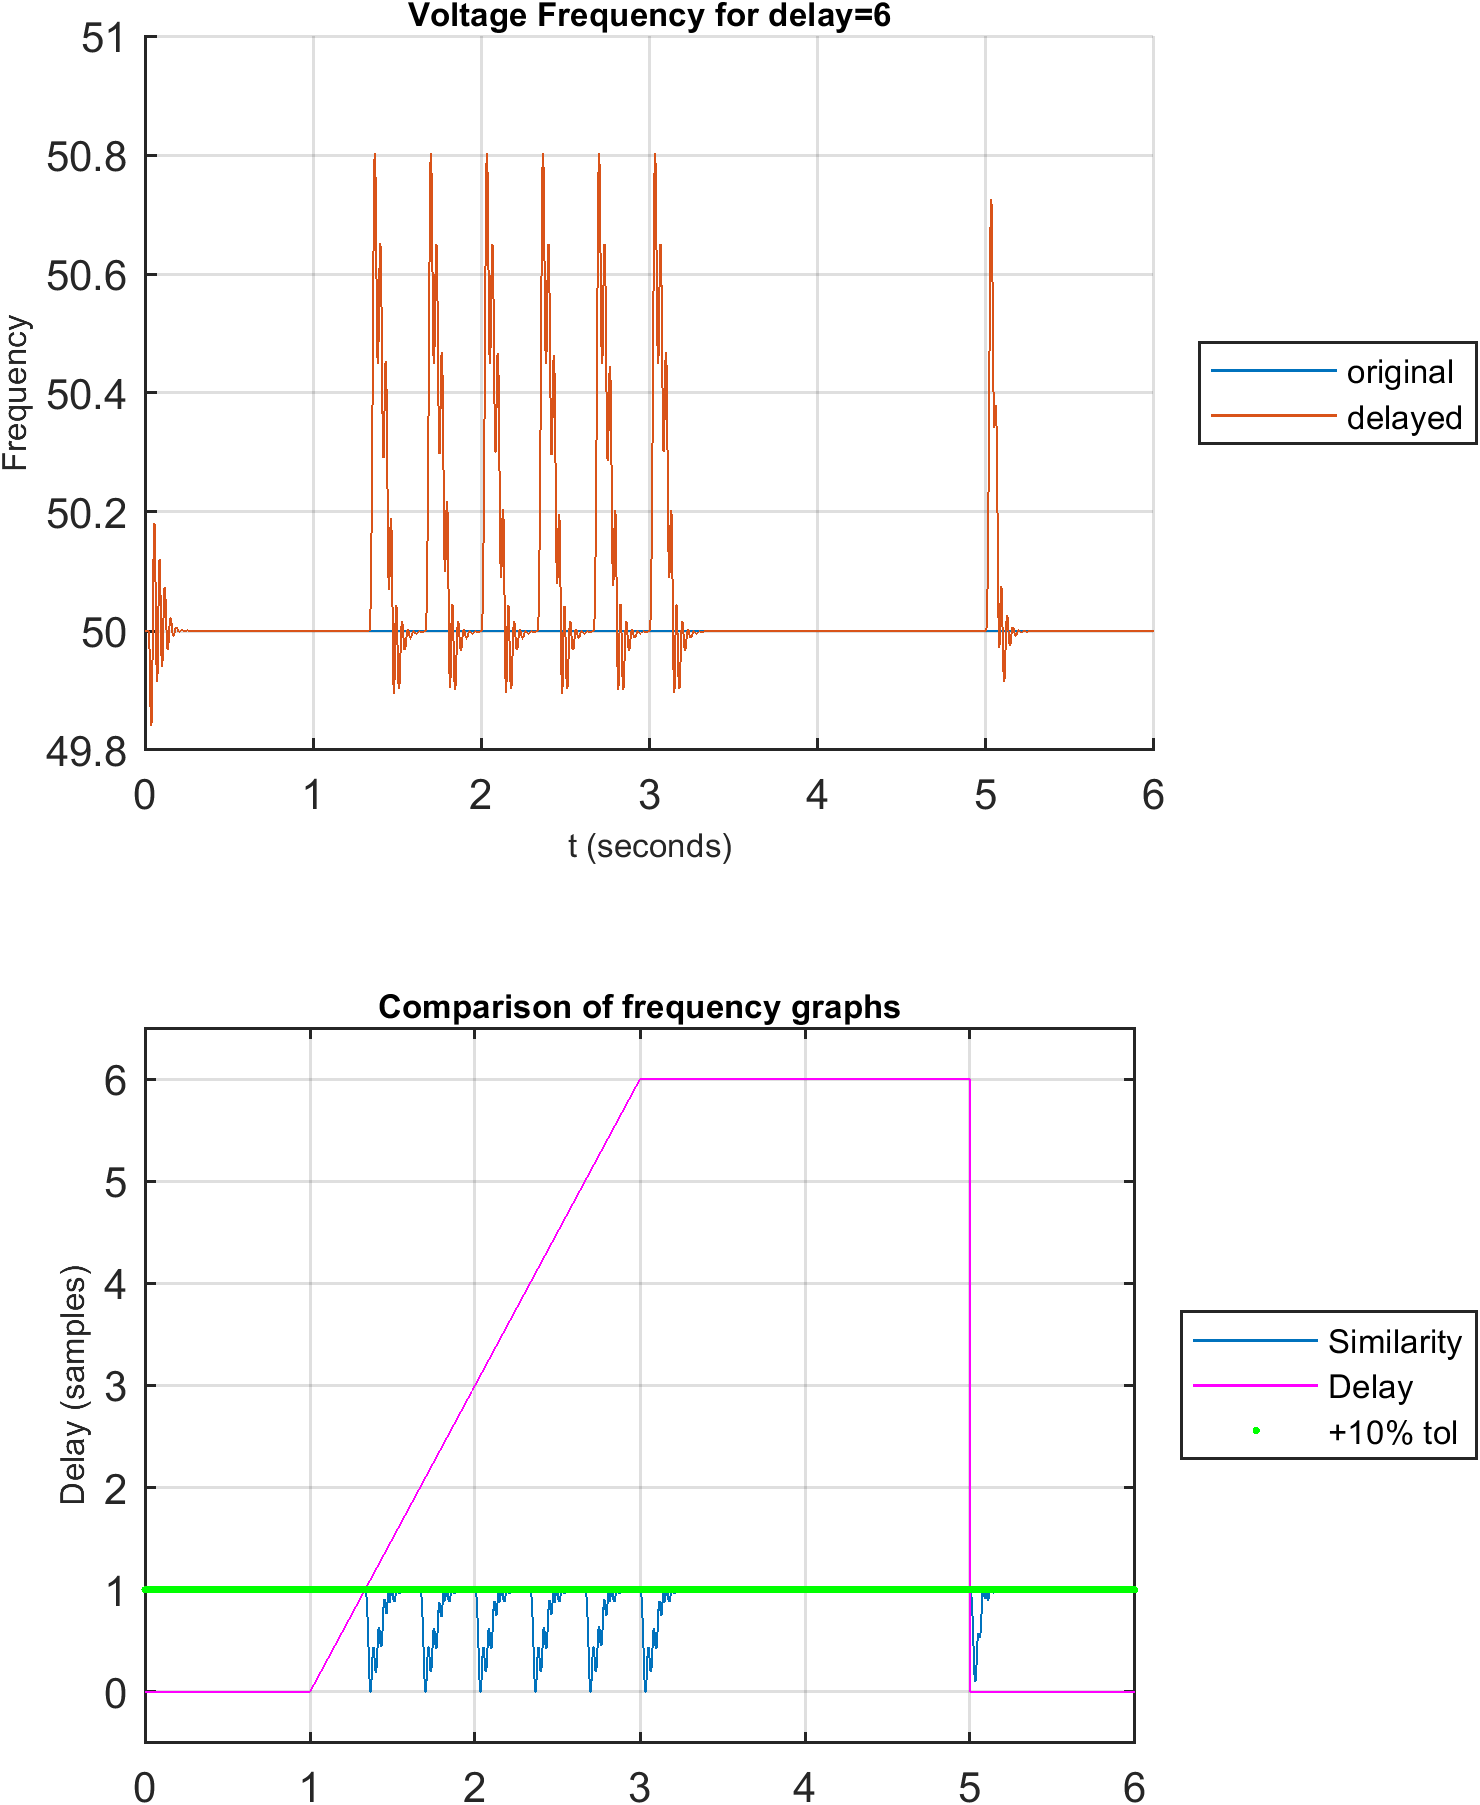
\includegraphics[width=\textwidth]{\locateResults/Frequency.png}    
         %\caption{frequency Output}
         \label{fig:PMUsim-Sqa2Freq}
        \caption{Frequency component output}
 
\end{figure}


